\chapter{The Analysis Lattice}
Inspired by TAJS we have a lattice for abstract values, $Value$, from which we build a lattice for abstract objects, $Object$. These two lattices are the main building blocks for the lattice of abstract states, $State$. Our analysis lattice is the lattice which for each program point (i.e. for each CFG node) tells the abstract state of that program point. Furthermore the analysis lattice tells the call graph of the CFG.

\section{Abstract Values}
The concrete lattices follows below.

\begin{eqnarray*}
Value = & Undefined \times None \times NotImplemented \times Ellipsis \\
        & \times Boolean \times Integer \times Float \times Long \\
        & \times Complex \times String \times P(ObjectLabel)
\end{eqnarray*}

The value lattice is used to tell the value of a temporary variable (see the lattice $Stack$), and a property on an object (see the lattice $Object$). The $Undefined$, $NotImplemented$, $Ellipsis$ and $None$ lattices all contains two nodes, top and bottom. $NotImplemented$ is a constant in Python that is used sometimes when a function is not supported. $Ellipsis$ is another constant which represents $\dots$ in Python, this constnat is used when indexing using intervals. In Python when a function does not contain a return statement, the constant \inlinecode{None}\cite{pyref.constants} is returned by default, e.g.:

\begin{listing}[H]
	\begin{minted}[linenos]{python}
def a(): pass
a() is None // true
	\end{minted}
	\caption{Constant None}\label{code:NoneExample}
\end{listing}

\begin{wrapfigure}{r}{0.5\textwidth}
	\vspace{-20pt}
	\begin{center}
		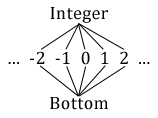
\includegraphics[width=0.48\textwidth]{images/integer-lattice.png}
	\end{center}
	\vspace{-10pt}
	\caption{The integer lattice}
	\label{fig:latticeInteger}
	\vspace{-10pt}
\end{wrapfigure}

Contrary to JavaScript, Python supports integers, floats, longs and complex numbers, so we have separate lattices for those. Note that $Complex = Float \times Float$, since a complex number in Python is represented using a float for the real and imaginary part, respectively \cite{pyref.stdtypes}. The Integer lattice is defined here in figure \ref{fig:latticeInteger}. The $Float$, $Long$ and $String$ lattices are defined in similar ways. Finally, a value can of course also be a pointer to an object on the heap, which we model in the $Value$ lattice by having a power set\footnote{All our power sets are ordered by subset inclusion.} of object labels, $P(ObjectLabel)$.


\section{Abstract State}
We use the following lattice to model abstract state:

\begin{equation*}
State = Heap \times Stack
\end{equation*}

In the following sections the $Heap$ and $Stack$ lattice will be described, but first it is necessary to look at the $Object$ lattice:

\begin{equation*}
Object = (PropertyName \rightarrow Value \times Global) \times P(ObjectLabel^{*})
\end{equation*}

Having made special lattices for the 'primitive' objects there is still a need to handle the more complex objects such as function objects. As with JavaScript you can augment objects with properties at runtime, so the lattice needs to accommodate this dynamic behavior, so we use a map from property names to values. For some objects it is required to track the scope in which they were defined, to model the closure they are evaluated in. Thus the object lattice is the product between object values and a scope chain modelled as a list of object labels.


\section{The Heap}
\begin{equation*}
Heap = (ObjectLabel \rightarrow Object)
\end{equation*}

The heap is modelled by a map from object labels to an object value. We found it benefitial to distinguish between different types of objects but still handle them in the same way in the heap. To achieve this we made several different subclasses to the object label object, e.g. function object, which besides its name also holds a reference to the CFG node that is the entry node for that function.


\section{The Stack}
The $Stack$ lattice is defined as:

\begin{equation*}
Stack = (TempVar \rightarrow Value) \times P(ObjectLabel^{*})
\end{equation*}

For each temporary variable we specify the value of that particular temporary variable. The power set $P(ObjectLabel^{*})$ specifies the scope chain ($ObjectLabel^{*}$). The head element in the scope chain determines which object on the heap, local variable writes should we written to. For instance we will for each program have an object on the heap, that models the module/top-level script environment \inlinecode{\_\_main\_\_}\cite{pyref.main} (this is what corresponds to the global object in JavaScript). Whenever an assignment to a variable occurs in the top-level scripting environment, e.g. \inlinecode{x=10}, the variable \inlinecode{x} is set as a property mapping to the integer 10 on the \inlinecode{\_\_main\_\_} object in the heap.

The scope chain specifies where to look in case of e.g. reading a variable that is not present on the variable object. The following simple example can be used to illustrate this:

\begin{listing}[H]
	\begin{minted}[linenos]{python}
x = 10
def a():
	return x
a() # 10
	\end{minted}
\caption{Scope example}\label{code:ScopeExample}
\end{listing}

For this particular scope example we will have the following objects on the heap:

\begin{enumerate}
  \item The \inlinecode{\_\_main\_\_} object,
  \item The object of the function \inlinecode{a},
  \item The function wrapper object of \inlinecode{a}, and
  \item The scope object of \inlinecode{a} (which is an object similar to the \inlinecode{\_\_main\_\_} object, i.e. an object where local variables are written onto).
\end{enumerate}

When entering the function (calling it) the scope object of the function a (or more precise, its label) will be pushed onto the current scope chain (which at the function call will be the list containing the \inlinecode{\_\_main\_\_} object). When the variable \inlinecode{x} is read, \inlinecode{x} is looked up in the scope chain starting from the head of it. For this particular example \inlinecode{x} is found on the \inlinecode{\_\_main\_\_} object. In the next chapter we describe our work towards handling functions including why we need these three different kinds of objects on the heap. Handling functions of course includes populating the call graph such that the CFG becomes interprocedural.

\begin{eqnarray*}
CallGraph = & (Node \times Node) \\
Analysis = & (Node \rightarrow State) \times CallGraph
\end{eqnarray*}
